% Abstract for this chapter
%
%**********************************************************************

%%%%%%%%%%%%%%%%%%%%%%%%%%%%%%%%%%%%%%%%%%%
\section{Reactionless motion control}
%%%%%%%%%%%%%%%%%%%%%%%%%%%%%%%%%%%%%%%%%%%
We consider a free-flying space robot model consisting of a satellite base and a serial manipulator arm
of $n$-DoF.
In space environment,
it is known that linear and angular momenta are conserved when there is no external force.
Actually,
the gravity gradient torque and solar radiation force violate this conservation.
However,
since the duration time of space robot missions is relatively short,
we can assume that the momenta are conserved.
Motion of a free-floating space robot is described via the spatial momentum conservation law as follows:
% 
% ---------------------------------------------------------------------
\begin{align}
  \bmat{\bm{p} \\ \bm{l}_{B}} = \bmat{\bm{M}_{v} & \bm{M}_{v\omega} \\ \bm{M}_{v \omega}^{T} & \bm{M}_{\omega}}
  \bmat{\bm{v}_{b} \\ \bm{\omega}_{b}} 
  +
  \bmat{\bm{M}_{vm} \\ \bm{M}_{\omega m}}\thd\label{eq:SPA_MOM_SP}
  % +
  % \bmat{\bm{0}\\\bm{r}_{b}\times \bm{p}}\label{eq:SPA_MOM_SP}
\end{align} 
% ---------------------------------------------------------------------
%
In this case, the link part represents a manipulator.
Hence, we make use of the subscript $(\circ)_{m}$ to represent ``manipulator''.

For free-flying space manipulators,
the angular momentum conservation law, especially,
is of primary importance.
Indeed, it has been noted that even slight variations of the base attitude may cause a failure
in the communication between the robot and the ground control center.
The angular momentum conservation law can be written in the following form, when zero initial momentum 
is assumed:
% 
% ---------------------------------------------------------------------
\begin{align}
  \bm{l}_{B} = \tbm{M}_{\omega}\bm{\omega}_{b} + \tbm{M}_{\omega m}\thd
\end{align} 
% ---------------------------------------------------------------------
%
where the notation $\tilde{(\circ)}$ represents a quantity that includes the base linear motion effect:
$\tbm{M}_{\omega} = \bm{M}_{\omega} - \bm{M}_{v\omega}^{T}\bm{M}_{v}^{-1}\bm{M}_{v\omega}$,
$\tbm{M}_{\omega m} = \bm{M}_{\omega m} - \bm{M}_{v\omega}^{T}\bm{M}_{v}^{-1}\bm{M}_{vm}$.
In the above equation,
the first term on the r.h.s.\ is the partial angular momentum stemming from base rotation.
The second term results from manipulator motion:
it represents the base disturbance in terms of momentum and is referred to as the 
\textit{coupling angular momentum} \cite{Nenchev1999a}.
% Finally,
% the third term represents the angular momentum stored in the reaction wheels.
% For the sake of simplicity, zero initial momenta are assumed without losing generality, hereafter.

To deal with the reaction problem,
reactionless motion control can be a useful approach.
Reactionless motions are variations of the manipulator configuration
that conserve a zero initial base angular momentum throughout a manipulator motion.
As explained already in \cha{BASIC},
these motions are obtained from the null-space vectors of the coupling inertia matrix.
Then, reactionless motion velocities are obtained as:
%
% ---------------------------------------------------------------------
\begin{align}
  \thd = \bm{P}_{RNS}\thd_{a}\label{eq:RNS_VELO}
\end{align}
% ---------------------------------------------------------------------
%
The velocities, of course, satisfy the following equation:
%
% ---------------------------------------------------------------------
\begin{align}
  \tbm{M}_{\omega m}\thd = \bm{0}\label{eq:RNS_CONST}
\end{align}
% ---------------------------------------------------------------------
%
The above equation implies the reactionless constraint.

Because $\thd_{a}$ is projected onto $\mathrm{ker}(\tbm{M}_{\omega m})$,
any values of $\thd_{a}$ satisfy the reactionless constraint \eq{RNS_CONST}.
The main concern of this study is how to make use of reactionless motions in practice.
Before proceeding with the discussion of the practical usages,
we should examine the features of reactionless motion.
The following section provides an analysis on reactionless motion with a planar model.



%%%%%%%%%%%%%%%%%%%%%%%%%%%%%%%%%%%%%%%%%%%%%%%%%%%%%%%%
\section{Qualitative study of reactionless motion}
%%%%%%%%%%%%%%%%%%%%%%%%%%%%%%%%%%%%%%%%%%%%%%%%%%%%%%%%
%%%%%%%%%%%%%%%%%%%%%%%%%%%%%%%%%%%%%%%%%%%%%%%
\subsection{Vector field of reactionless motion}
\label{sec:ANALYSIS_FIXED}
%%%%%%%%%%%%%%%%%%%%%%%%%%%%%%%%%%%%%%%%%%%%%%%
%
% ---------------------------------------------------------------------
\begin{figure}[t]
  \centering
  \begin{minipage}[t]{0.36\linewidth}
    \centering
    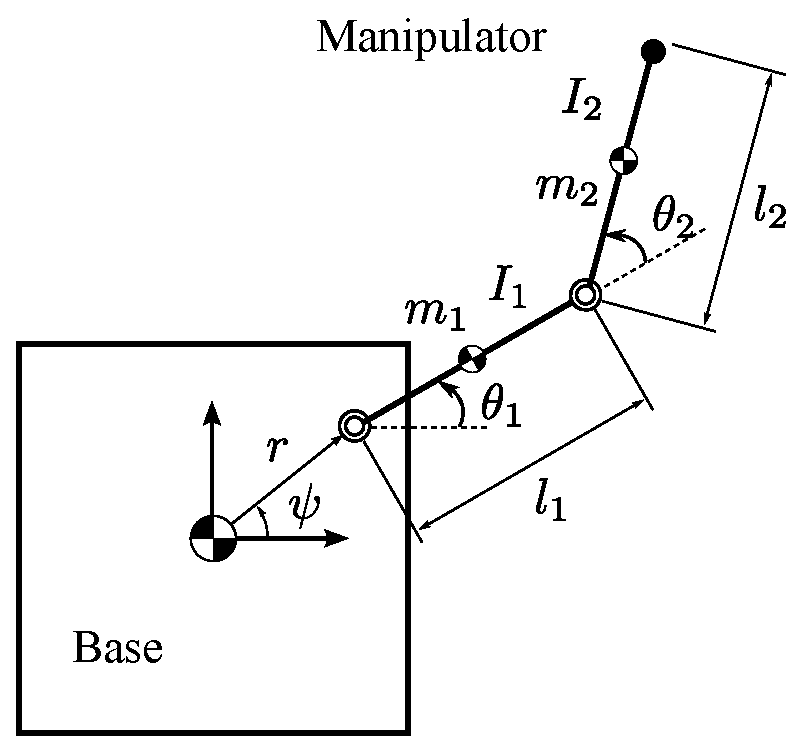
\includegraphics[width=1.0\linewidth]{fig/chapter3/planar/FF2RModel.eps}
  \end{minipage}
  \hspace{4mm}
  \begin{minipage}[t]{0.30\linewidth}
    \centering
    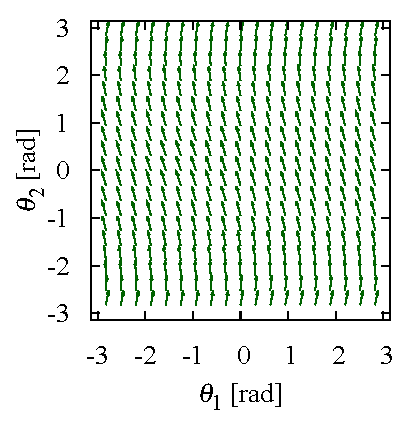
\includegraphics[width=1.0\linewidth]{fig/chapter3/planar/vectorField.eps}
  \end{minipage}
  \caption{A planar two-DoF space manipulator model with $m_{i} = 100\unit{kg}$,
  $l_{i} = 1.0\unit{m}$ ($i = 1, 2$); the base mass is $m_{b} = 1000\unit{kg}$.
  The vector field is obtain with $r = 0\unit{m}$.}
  \label{fig:FF2R}
\end{figure}
% ---------------------------------------------------------------------
%
Existing results from reactionless motion control have been reported in the Introduction. 
There are, however, some  characteristics of reactionless motion that have not been mentioned so far.

Consider first a simple planar two-DoF manipulator on a satellite base, as shown in \fig{FF2R}.
This model is the simplest one with the capability of reactionless motion generation.
Reactionless motion with this model can be represented as follows:
%
% ---------------------------------------------------------------------
\begin{align}
  \thd = b\bm{n}(\th)\label{eq:RNSSYST}
\end{align}
% ---------------------------------------------------------------------
%
where $\bm{n}(\th)\R{2}$ is the only generic null-space vector in the kernel 
of the coupling inertia matrix, and $b$ is an arbitrary scalar dimensioned as joint velocity.
$\bm{n}(\th)$ can be uniquely obtained through appropriate methods,
i.e.\ Singular Value Decomposition (SVD) or the co-factor method.
We assume that $\bm{n}(\th)$ is already normalized,
and $b$ is a time-independent constant scalar, for the sake of simplicity.
Hence, \eq{RNSSYST} can be regarded as an autonomous nonlinear system.
The right hand side in \eq{RNSSYST} defines the vector field of reactionless motion
in joint space.

%We examine the properties of reactionless motion with the above vector field.
For the sake of simplicity, we assume that the manipulator is attached at the CoM of the base.
The mass and inertia moment of the base are $m_{b} = 1000\unit{kg}$, ${I}_{b} = 667\unit{kgm^{2}}$;
the length, mass and inertia moments of the links are $l_{i} = 1.0\unit{m}$,
$m_{i} = 100\unit{kg}$ and ${I}_{i} = 8.33\unit{kgm^{2}}$ ($i = 1,2$), respectively.
The resultant vector field is depicted in \fig{FF2R}. 
Because the manipulator is attached symmetrically,
the vector field has rotational symmetry w.r.t.\ Joint 1.
From the vector field, an important property becomes apparent:  reactionless motion is predominantly 
composed of Joint 2 motion. 
Because reactionless motion  conserves  angular momentum at zero (or at a constant),
motion in the joints that induce a large angular momentum cannot variate significantly.
With this model, the angular momentum induced by Joint 1 motion must be larger than
that of Joint 2  due to the large inertia moment and the long moment arm. 
As a result, the above mentioned behavior is observed.

%%%%%%%%%%%%%%%%%%%%%%%%%%%%%%%%%%%%%%%%%%%%%%%
\subsection{Fixed point and bifurcation}
\label{sec:ANALYSIS_FIXED}
%%%%%%%%%%%%%%%%%%%%%%%%%%%%%%%%%%%%%%%%%%%%%%%
In the above example, the system does not have any fixed points.
It turns out, however, that the variation of the manipulator attachment position
induces such points and moreover, a bifurcation can be observed.
The attachment position is made variable according to:
%
% ---------------------------------------------------------------------
\begin{align}
  \begin{bmatrix}
    x_{a}\\
    y_{a}
  \end{bmatrix}
  =
  r
  \begin{bmatrix}
    \cos\psi\\
    \sin\psi
  \end{bmatrix}
\end{align}
% ---------------------------------------------------------------------
%
where %$(\circ)_{a}$ is the coordinate of the attachment position,
$r$ is the distance between the attachment position and the base CoM,
and $\psi$ is the angle as shown in \fig{FF2R}.
Among these parameters, $r$ plays an important role as a \textit{bifurcation parameter} in this system.
Note that we can assume $\psi = 0$ because this parameter does not influence the topological structure
of the system due to the existing rotational symmetry. Hence, it is sufficient to variate 
the attachment position along the $x$-axis of the base frame.

%
% --------------------------------------------------------------------
\begin{figure}[t]
  \centering
  \begin{minipage}[t]{0.30\linewidth}
    \centering
    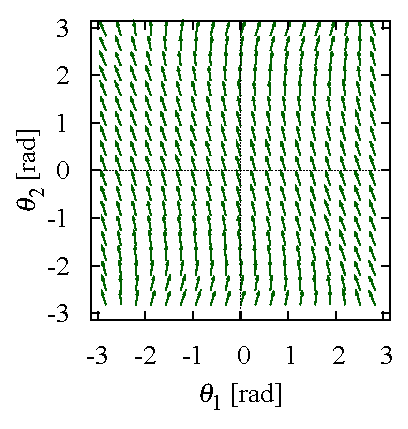
\includegraphics[width=1.0\linewidth]{fig/chapter3/planar/0.5.eps}
    \hspace{2mm}
  \end{minipage}
  \begin{minipage}[t]{0.30\linewidth}
    \centering
    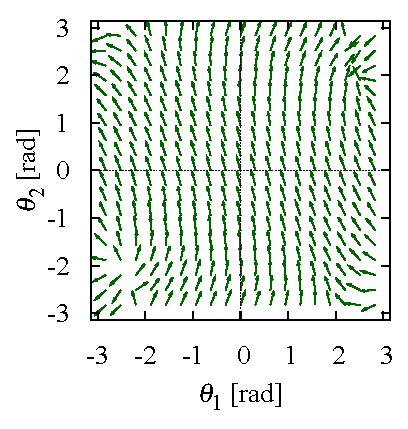
\includegraphics[width=1.0\linewidth]{fig/chapter3/planar/0.945.eps}
    \hspace{2mm}
  \end{minipage}
  \begin{minipage}[t]{0.30\linewidth}
    \centering
    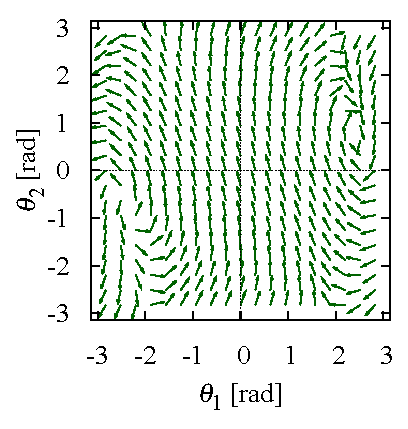
\includegraphics[width=1.0\linewidth]{fig/chapter3/planar/1.5.eps}
    \hspace{2mm}
  \end{minipage}\\
  \vspace{-3mm}
  \begin{minipage}[t]{0.30\linewidth}
    \centering
    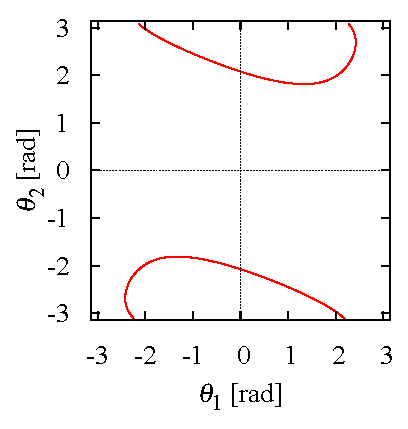
\includegraphics[width=1.0\linewidth]{fig/chapter3/planar/0.5_nullclines.eps}
    \footnotesize\par{(a)}
    \hspace{2mm}
  \end{minipage}
  \begin{minipage}[t]{0.30\linewidth}
    \centering
    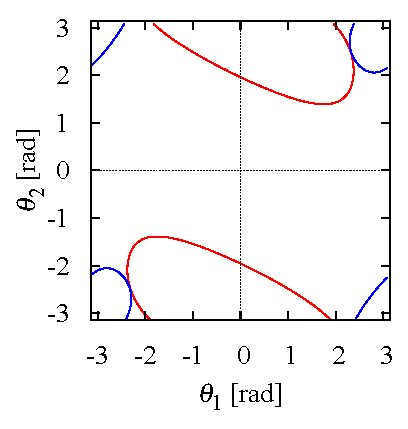
\includegraphics[width=1.0\linewidth]{fig/chapter3/planar/0.945_nullclines.eps}
    \footnotesize\par{(b)}
    \hspace{2mm}
  \end{minipage}
  \begin{minipage}[t]{0.30\linewidth}
    \centering
    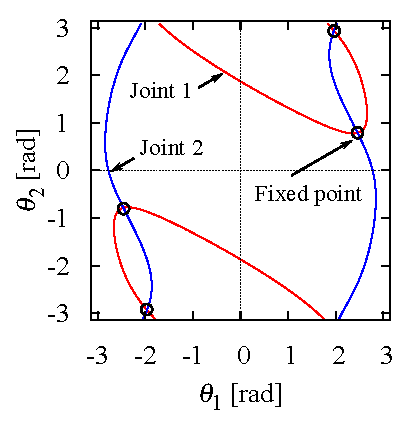
\includegraphics[width=1.0\linewidth]{fig/chapter3/planar/1.5_nullclines.eps}
    \footnotesize\par{(c)}
    \hspace{2mm}
  \end{minipage}
  \caption{The vector field and nullclines for each joint direction when $r$ variates as: 
    (a) $r = 0.5\unit{m}$, (b) $r = 0.945\unit{m}$ and (c) $r = 1.5\unit{m}$.}
    \label{fig:BIF_VEC}
\end{figure}
% --------------------------------------------------------------------
%
In \fig{BIF_VEC},  the vector field and nullclines for  several values of $r$ are shown.
In the figures, the upper part represents the vector field and
the lower part depicts nullclines for each joint direction:
the lines in red are for Joint 1, those  in blue are  for Joint 2. 
When $r = 0.5\unit{m}$, we can see that there is no fixed point,
because the motion of Joint 2 never stops at any point in joint space.
On the other hand, the occurrence of a bifurcation can be observed when 
$r \approx 0.945\unit{m}$.
Then, two fixed points are created at the intersection points of the two nullclines.
Further increase of the bifurcation parameter ($r = 1.5\unit{m}$) 
leads to separation of the created fixed points. 
Finally, when $r \rightarrow \infty$, two of the fixed points converge to
$\theta_{2} \rightarrow 0\unit{rad}$ and
the rest  to $\theta_{2} \rightarrow \pm\pi\unit{rad}$.

%%%%%%%%%%%%%%%%%%%%%%%%%%%%%%%%%%%%%%%%%%%%%%%%%%%%%%%%%%%%%%%%
\subsection{Rank deficiency of the coupling inertia matrix}
\label{sec:ANALYSIS_SING}
%%%%%%%%%%%%%%%%%%%%%%%%%%%%%%%%%%%%%%%%%%%%%%%%%%%%%%%%%%%%%%%%
In above discussion, we clarified the existence of fixed points with regard to reactionless motion.
This phenomenon is related to the rank deficiency of the coupling inertia matrix.
In contrast to kinematic singularities, the singularities of the coupling inertia matrix have 
not been discussed, so far. We provide some insight with the planar model mentioned above.

%
% ---------------------------------------------------------------------
\begin{figure}[t]
  \centering
  \begin{minipage}[t]{0.42\linewidth}
    \centering
    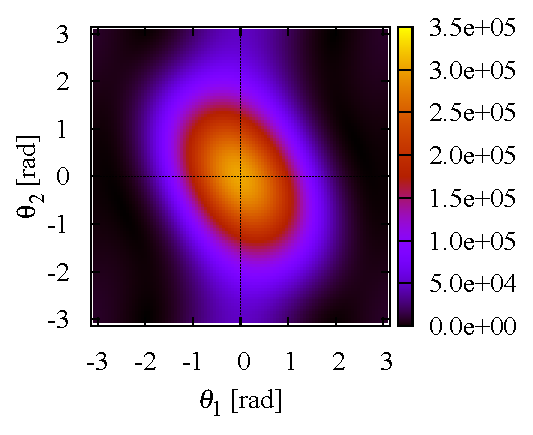
\includegraphics[width=1.0\linewidth]{fig/chapter3/planar/determinant.eps}
    \footnotesize\par{(a)}
  \end{minipage}
  \hspace{1mm}
  \begin{minipage}[t]{0.38\linewidth}
    \centering
    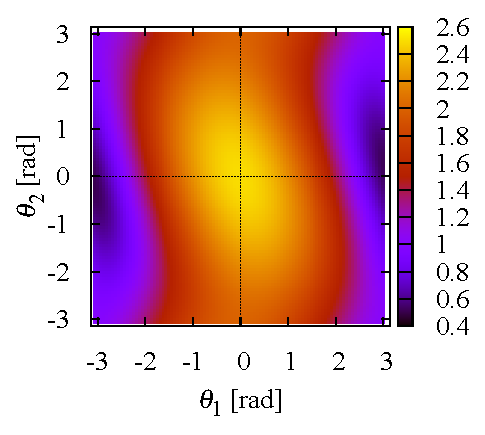
\includegraphics[width=1.0\linewidth]{fig/chapter3/planar/com.eps}
    \footnotesize\par{(b)}
  \end{minipage}
  \caption{This figure shows the determinant of $(\bm{M}_{\omega m}\tbm{M}_{\omega m}^{T})$ and
  the distance between the manipulator CoM and the base one as color map:
  (a) $\mathrm{det}(\tbm{M}_{\omega m}\tbm{M}_{\omega m})$ and (b) the distance between the manipulator CoM and the base one.}
  \label{fig:DET_FF2R}
\end{figure}
% ---------------------------------------------------------------------
%
Determinant $\det (\tbm{M}_{\omega m}\tbm{M}_{\omega m}^{T})$
for  $r = 1.5\unit{m}$ is shown as a colored map in \fig{DET_FF2R}~(a).
The determinant takes large values at the bright areas, 
while the most dark area represents the singularities.
It is apparent that the determinant takes its maximum value at $\th = \bm 0$.
This is an extended-arm configuration s.t.\ the manipulator CoM is located farthest away 
from the base CoM. Note that determinant $\det(\tbm{M}_{\omega m}\tbm{M}_{\omega m}^{T})$ can be 
related to the distance between the two CoMs as shown in
%, which is depicted on the joint space plane in  
\fig{DET_FF2R}~(b). Comparing the two plots in \fig{DET_FF2R}, it can be seen that the determinant
takes large values whenever the distance is relatively large. Large CoM distance yields 
large  moment of  momentum and hence, large magnitude of the coupling angular momentum.  
Furthermore, note that there is no fixed point within the area where the distance is large.
In the case of a spatial model, the directions  of the joint axes play an 
important role in addition to the above qualitative characteristics. 

%%%%%%%%%%%%%%%%%%%%%
\section{Summary}
%%%%%%%%%%%%%%%%%%%%%
In this chapter,
we described some characters of reactionless motion with a planar model.
From a qualitative analysis,
we found out that the manipulator attachment position plays an important role
in terms of bifurcation.
Then, through vector field,
we confirmed that the fixed points of reactionless motion are generated,
increasing the length between the manipulator attachment position and the base CoM.







%**********************************************************************
%
%
%%% Local Variables:
%%% mode: latex
%%% TeX-master: "./main"
%%% End: